\chapter{\textbf{Proposed Method}}
\label{chapter: Proposed Method}
In this chapter, we present the design of \myalgorithm, our proposed bandit-based algorithm for online SFC orchestration at the edge.

We first present the contextual combinatorial bandit formulation~\cite{C^2MAB} of the chain placement problem by characterizing the environment with a set of \emph{arms} (\ie\ placement options) and specifying their relations in subsection~\ref{section_bandit_formulation}.
The formulation reduces the bandit solution's computational complexity and allows the user to handle the uncertainty in the environment and through repeated interactions to find efficient service placement and resource allocation schemes. Specifically, the context allows the user to incorporate the available information into the resource allocation procedure (\eg\ demand). The combinatorial formulation allows the user to focus on the primitive options (\ie\ servers and links) during the learning procedure, which significantly reduces the problem space. Otherwise, the user would be forced to consider all the solutions, which are exponential in terms of the number of servers and links (\eg\ all the different paths in the network). 
Then, we show how to reduce the uncertainty about the quality
of arms and use the result to compute a service efficiently
placement by dynamic programming, which is presented in subsection~\ref{sec:placement algorithm}


%In this section, we present the design of \myalgorithm, our proposed bandit-based algorithm for online SFC orchestration at the edge. To reduce the computational complexity of the bandit solution, we apply the contextual bandit formulation~\cite{C^2MAB} by characterizing the environment with a set of \emph{arms} (\ie\ placement options) and specifying their relations in subsection~\ref{section_bandit_formulation}.
%%
%Then, we show how to reduce the uncertainty about the quality of arms and use the result to efficiently compute a service placement by dynamic programming in subsection~\ref{subsection_dynamic_programming}.


\subsection{Bandit Formulation}
\label{section_bandit_formulation}
At the beginning of each timeslot $t$,
user-side information such as their service demands $\lambda(t)$ during the timeslot, the current location $\beta(t)$, and the placement of their service chain in the previous timeslot(\ie\ $x_n^s(t-1)$) is known. In contrast, the system-level information such as processing and bandwidth capacity of servers and links are not accessible, thereby are required to be learned by the user. 
%
Therefore, to learn about the environment, we consider each server and link as an option that can be used for placing a service, which is analogous to the concept of \emph{arm} in bandit theory. The available options in each timeslot are defined to be $O_{t}\subseteq \mc{L}\cup\mc{N}$, which is the set of all links, user's device, edge servers, and the remote cloud. At the beginning of each timeslot, based on the information learned so far, the user selects a subset of feasible options for the service chain's placement and minimizes the end-to-end delay. At the end of each timeslot, the user observes each option's contribution to the delay objective. Specifically, for each selected option $o\in O_{t}$, the user observes some value $\delta_{o}(t)$. This value is only a noisy estimate of the true value of the option $o\in O_{t}$. Our goal is to quickly and efficiently estimate the true values of delays incurred by each option.
%
According to our delay formulation, each option contributes \emph{linearly} to the user's perceived end-to-end delay. Following the framework of contextual bandits, we assume that in each timeslot $t$, the significance of each option depends only on an unknown system parameter vector $\theta$ and a contextual feature vector $\pmb{\chi}_{o}(t)$ that is fully known to the user. For example, the edge server capacities are unknown parameters but the user's current location is a known contextual feature.
%
Thus, the observed value $\delta_{o}(t)$ is characterized as follows:
\begin{gather}
	\delta_{o}(t) = \theta^{\intercal} \times \pmb{\chi}_{o}(t) + \epsilon_{o}(t),
\end{gather}
where, $\epsilon_{o}(t)$ is a zero-mean random variable representing the noise delay in the network. 
%

Note that the user can select arm $o$ as a part of service placement resources but only observes the resulting delay $\delta_{o}(t)$ at the end of the timeslot. Specifically, the user, in each timeslot, using the historical information, should select a subset of options $O_{t}\subseteq \mc{L}\cup\mc{N}$ that (1) is feasible for the placement of the service chain and (2) minimizes the overall delay perceived by the user. The user's goal is to minimize the expected cumulative delay in the period of service placement, which is defined as,
\begin{gather}
	\mathbb{E}\left[\sum_{t\in\mc{T}} \sum_{o\in O_{t}} \delta_{o}(t)\right].
\end{gather}

In the following, we fully describe the system parameter vector
$\theta$ and contextual feature vector $\pmb{\chi}_{o}(t)$.

\cat{System Parameters}
The parameter vector of the system (which is unknown to the user) is composed of four sub-vectors, where each sub-vector contains parameters that are related to a specific type of delay.
\begin{enumerate}[leftmargin=*]
	\item $\theta_{c}$ is the sub-vector of parameters that determine the processing delay based on the number of CPU cores in each computing node:
	\begin{gather}
		\theta_{c} = [\textstyle\frac{1}{c_{n}}, \quad \forall n\in\mc{N}]. 
	\end{gather}
	\item $\theta_{b}$ is the sub-vector of parameters that determine the transmission delay based on the bandwidth of links:
	\begin{gather}
		\theta_{b} = [\textstyle\frac{1}{b_{\ell}}, \quad \forall \ell\in\mc{L}].
	\end{gather}
	\item $\theta_{d}$ is the sub-vector of parameters that determine the propagation delay:
	\begin{gather}
		\theta_{d} = [d_{\ell}, \quad \forall \ell\in\mc{L}].
	\end{gather}
	\item $\theta_{\rho}$ is the sub-vector of parameters that determine the service migration delay:
	\begin{gather}
		\theta_{\rho} = [\rho_{a,b}^{s}, \quad \forall a,b\in\mc{N}, s\in\mc{S}].
	\end{gather}
\end{enumerate}
Finally, it is possible to construct the system parameter vector $\theta$ from the concatenation of the aforementioned sub-vectors:
\begin{gather}
	\theta = \theta_{c} \oplus \theta_{b} \oplus \theta_{d} \oplus \theta_{\rho},
\end{gather}
where, $\oplus$ is the concatenation operator.


\cat{Notation}
In the following, we use the notation $1_p$ to represent an indicator function that is equal to $1$ when the logical predicate $p$ is true and is equal to $0$ otherwise. 

\cat{Contextual Features}
We define a contextual feature vector to represent the known information at the user's side for each placement option $o\in O_t$. Each option is either a link $o=\ell\in\mc{L}$ or a computation node $o=n\in\mc{N}$. Since the information about links and nodes are different, we define a feature vector for nodes and links separately. The contextual vector, similar to the parameter vector, comprises four sub-vectors that correspond to four types of delay. The link contextual sub-vectors are defined as follows:
\begin{enumerate}[leftmargin=*]	
	\item $\pmb{\chi}_{\ell}^{b}(t)$ is the sub-vector corresponding to the transmission delay. $\pmb{\chi}_{\ell}^{b}(t)$ contains contextual information about the user's transmission rate.
	\begin{gather}
		\pmb{\chi}_{\ell}^{b}(t) = [1_{\ell'=\ell,\exists n\in\mc{N}: \ell'\in \delta^{-}(n)}\lambda_{s}(t), \quad \forall \ell'\in\mc{L}].
	\end{gather}
	Note that if the user uses link $\ell$ to transfer the result of computation out of the computation node $n$, the multiplication of this sub-vector by the system parameter vector computes the expected transmission delay.
	\item When the user selects a link, its corresponding propagation delay is incurred. Thus, the contextual propagation delay sub-vector of link $\ell$, denoted by $\pmb{\chi}_{\ell}^{d}(t)$, is defined as:
	\begin{gather}
		\pmb{\chi}_{\ell}^{d}(t) = [1_{\ell'=\ell}, \quad \forall \ell'\in\mc{L}],
	\end{gather}
	Note that when this sub-vector is multiplied by the corresponding system sub-vector the propagation delay of $\ell$ is obtained.
	
	\item Since links have no effect on the computational and migration delays, the corresponding sub-vectors, denoted by $\pmb{\chi}_{\ell}^{c}(t)$ and $\pmb{\chi}_{\ell}^{\rho}(t)$, respectively, are zero vectors:
	\begin{gather}
		\pmb{\chi}_{\ell}^{c}(t) = [0, \quad \forall n\in\mc{N}], \\
		\pmb{\chi}_{\ell}^{\rho}(t) = [0, \quad \forall a,b\in\mc{N}, s'\in\mc{S}].
	\end{gather}
\end{enumerate}
Thus, the contextual feature vector of each link $\ell$ that is going to be used to route the traffic towards service $s\in\mc{S}$ is obtained from the concatenation of these sub-vectors:
\begin{gather}
	\pmb{\chi}_{\ell}(t) = \pmb{\chi}_{\ell}^{c}(t) \oplus \pmb{\chi}_{\ell}^{b}(t) \oplus \pmb{\chi}_{\ell}^{d}(t) \oplus \pmb{\chi}_{\ell}^{\rho}(t), 
\end{gather}
The contextual feature vector of each computation node is defined based on four sub-vectors as follows:
\begin{enumerate}[leftmargin=*]
	\item The contextual sub-vector of computation features, denoted by $\pmb{\chi}_{n}^{c}(t)$, is defined as follows: 
	\begin{gather}
		\pmb{\chi}_{n}^{c}(t) = [1_{n'=n}\times \pi_{s}\lambda_{s}(t), \quad \forall n'\in\mc{N}].
	\end{gather}
	Note that if we multiply this sub-vector by the sub-vector of system parameters for computation, the computation delay of running the service $s$ on node $n$ is obtained.
	\item The migration contextual sub-vector contains information about the placement of services in the previous timeslot.  We denote this sub-vector by $\pmb{\chi}_{n}^{\rho}(t)$ and define it as follows:
	\begin{gather}
		\pmb{\chi}_{n}^{\rho}(t) = [1_{s'=s,b=n}x_{a}^{s}(t-1), \quad \forall a,b\in\mc{N}, s'\in\mc{S}].
	\end{gather}
	%\hl{	Note that this sub-vector }
	\item Since computation nodes do not affect the transmission and propagation delays, the corresponding contextual feature sub-vectors, denoted by $\pmb{\chi}_{n}^{b}(t)$ and $\pmb{\chi}_{n}^{d}(t)$, respectively, are zero vectors: 
	\begin{gather}
		\pmb{\chi}_{n}^{b}(t) = [0, \quad \forall \ell\in\mc{L}], \\
		\pmb{\chi}_{n}^{d}(t) = [0, \quad \forall \ell\in\mc{L}].
	\end{gather}
\end{enumerate}
Finally, the contextual feature of each node $n$ where service $s\in\mc{S}$ is placed is obtained by concatenating the mentioned sub-vectors:
\begin{gather}
	\pmb{\chi}_{n}(t) = \pmb{\chi}_{n}^{c}(t) \oplus \pmb{\chi}_{n}^{b}(t) \oplus \pmb{\chi}_{n}^{d}(t) \oplus \pmb{\chi}_{n}^{\rho}(t), 
\end{gather}


\subsection{Placement Algorithm}
\label{sec:placement algorithm}
In this subsection, we present the design of our proposed bandit-based algorithm that efficiently estimates each arm's value, which is equivalent to the expected delay of each placement option.
Our proposed bandit-based algorithm for SFC placement on edge is summarized in Algorithm~\ref{alg:cccpa}, called \myalgorithm.
\myalgorithm\ repeatedly examines different placement strategies and adjusts the estimates based on the noisy feedback it receives from the system. Then, \myalgorithm\ uses the expected estimated delay values to compute a placement with the minimum end-to-end delay. \myalgorithm\ is outlined in  Algorithm~\ref{alg:cccpa}. \myalgorithm\ gets the service chain, the contextual features, and available nodes and links as the input. To estimate the expected delay for each placement option, the algorithm has to estimate the system parameter vector $\theta$. We use $\hat{\theta}(t)$ and $\hat{\delta}_o(t)$ to represent the estimated parameter vector and estimated delay for placement option $o$ at timeslot $t$. To compute these values, we applied the confidence bound-based algorithm in~\cite{C^2MAB}.

The algorithm starts with an initial estimate for the covariance matrix  $\pmb{V}_{0}$ and mean vector $\pmb{b}_{0}$ of system parameters expressed as follows (line~\ref{alg_bandedge_line_V0}-\ref{alg_bandedge_line_b0}),
\begin{gather}
	\pmb{V}_{0} \gets \pmb{I}_{d\times d}, \label{eqn:v_init} \\

	\pmb{b}_{0} \gets \pmb{0}_{d}, \label{eqn:b_init}.\end{gather}

In each timeslot, the estimated system parameter vector is obtained from the covariance matrix and the mean vector. The estimated system parameter vector is then used to compute the excepted delay of each placement option, which is expressed as follows (line~\ref{alg_bandedge_line_theta}-\ref{alg_bandedge_line_delta_bar}), 
\begin{gather}
	\hat{\theta}(t)
	\gets
	\pmb{V}_{t-1}^{-1}\pmb{b}_{t-1}, \label{eqn:theta_hat}\\
	\bar{\delta}_{o}(t)
	\gets
	\hat{\theta}(t)^{\intercal}
	\pmb{\chi}_{o}(t), \forall o \in O_t.
\end{gather}
Then, a lower bound for each delay values in computed as follows (line~\ref{alg_bandedge_line_delta_hat}),
\begin{gather}
	\hat{\delta}_{o}(t)
	\gets
	\bar{\delta}_{o}(t)
	-
	\sqrt{\pmb{\chi}_{o}(t)^{\intercal}\pmb{V}_{t}^{-1}\pmb{\chi}_{o}(t)}. 
	\label{eqn:delta_hat}
\end{gather}

Then, the algorithm selects a set of placement options $P_{t}$ at time $t$ based on a placement strategy, which is expressed as follows(line~\ref{alg_bandedge_line_place}),
\begin{gather}
	P_{t}\leftarrow \textbf{Place}(\hat{\delta}_{o}(t), \mc{S}[t]).
\end{gather}
The placement strategy, based on dynamic programming, is outlined in Algorithm~\ref{alg:DP_SFC}.

Finally, the computed placement is implemented and the algorithm observes the delay values
incurred as a result. The algorithm the update the covariance matrix
and the mean vector accordingly as follows (line~\ref{alg_bandedge_line_update_V}-\ref{alg_bandedge_line_update_b}),
\begin{gather}
	\pmb{V}_{t} \gets \pmb{V}_{t-1} + \sum_{{o}\in P_{t}} \pmb{\chi}_{o}(t)\pmb{\chi}_{o}(t)^{\intercal}, \label{eqn:v_update}\\
	\pmb{b}_{t} \gets \pmb{b}_{t-1} + \sum_{{o}\in P_{t}} \delta_{o}(t)\pmb{\chi}_{o}(t).\label{eqn:b_update}
\end{gather}
%The user, then, uses $\pmb{V}_{0}$ and $\pmb{b}_{0}$ as follows to compute new lower-bound estimates,
%\begin{gather}
%\hat{\theta}(t)
%\gets
%\pmb{V}_{t}^{-1}\pmb{b}_{t}, \label{eqn:theta_hat} \\
%\bar{\delta}_{n}(t)
%\gets
%\hat{\theta}(t)^{\intercal}
%\pmb{\chi}_{n}(t), \\
%\hat{\delta}_{n}(t)
%\gets
%\bar{\delta}_{n}(t)
%-
%c\sqrt{\pmb{\chi}_{n}(t)^{\intercal}\pmb{V}_{t}^{-1}\pmb{\chi}_{n}(t)}, \label{eqn:delta_hat}
%\end{gather}

\cat{Exploration vs Exploitation}
In online learning, \textit{Exploration} allows user to improve their knowledge about each arm that is likely to lead to a long-term benefit while \textit{Exploitation} allows user to exploit their current knowledge by choosing the current largest estimated arms. In equation~\ref{eqn:delta_hat}, $\bar{\delta}_{n}(t)$ denotes the current estimates at timeslot $t$ and therefore represent the exploitation, while $\sqrt{\pmb{\chi}_{n}(t)^{\intercal}\pmb{V}_{t}^{-1}\pmb{\chi}_{n}(t)}$ denotes the adjustment made on each arm and therefore represent exploration. Additionally, we associate
a constant ratio $c$ to exploration term to determine the exploration-exploitation level, refer to as \textit{exploration ratio}.\ \eg, bigger $c$ leads to a smaller lower bound on the estimates and encourages exploration, smaller $c$ leads to a larger lower bound and encourages exploitation. We further evaluate the effect of the exploration ratio $c$ in section~\ref{eval:explorationratio}.
\begin{algorithm}[t]
	%\fontsize{12}{12}\selectfont
	\DontPrintSemicolon
	\caption{\textbf{\myalgorithm}: \textbf{Cha}i\textbf{n} Orchestrator at the Ed\textbf{ge}}
	\label{alg:cccpa}
	\SetKwInput{kwInit}{Init}
	\textbf{Input}: $\mc{N}, \mc{L}, \mc{S},\pmb{\chi} $\\
	$\pmb{V}_{0} \gets \pmb{I}_{d\times d}$ \label{alg_bandedge_line_V0} \\
	$\pmb{b}_{0} \gets \pmb{0}_{d}$ \label{alg_bandedge_line_b0} \\
	\For{$t\in \mc{T}$}{
		$\hat{\theta}(t)
		\gets
		\pmb{V}_{t-1}^{-1}\pmb{b}_{t-1}$ \label{alg_bandedge_line_theta} \\
		$\bar{\delta}_{o}(t)
		\gets
		\hat{\theta}(t)^{\intercal}
		\pmb{\chi}_{o}(t), \forall o \in O_t$ \label{alg_bandedge_line_delta_bar} \\
		$\hat{\delta}_{o}(t)
		\gets
		\bar{\delta}_{o}(t)
		-
		\sqrt{\pmb{\chi}_{o}(t)^{\intercal}\pmb{V}_{t}^{-1}\pmb{\chi}_{o}(t)}$ \label{alg_bandedge_line_delta_hat} \\
		$P_{t}\leftarrow \textbf{Place}(\hat{\delta}_{o}(t), \mc{S}[t])$ \label{alg_bandedge_line_place} \\
		$\pmb{V}_{t} \gets \pmb{V}_{t-1} + \sum_{{o}\in P_{t}} \pmb{\chi}_{o}(t)\pmb{\chi}_{o}(t)^{\intercal}$ \label{alg_bandedge_line_update_V} \\
		$\pmb{b}_{t} \gets \pmb{b}_{t-1} + \sum_{{o}\in P_{t}} \delta_{o}(t)\pmb{\chi}_{o}(t)$ \label{alg_bandedge_line_update_b} \\
	}
\end{algorithm}

%\cat{Proposed Algorithm} Our proposed bandit based algorithm for SFC placement on Edge is summarized in Algorithm~\ref{alg:cccpa}, we call it \textit{\myalgorithm} 
\cat{SFC placement algorithm}The SFC placement algorithm, presented in Algorithm~\ref{alg:dplace} is based on the dynamic programming (DP) principle, which, given the delay estimates $\hat{\delta}_{o}(t)$ and required service set $\mc{S}[t]$,  calculates the optimal resource allocation in polynomial time by defining the cost of an optimal solution recursively in a bottom-up fashion. DP finds the optimal solution by starting from placing one single service and successively moving to next service while taking the previous solutions into account. There are three recurrence relations for the minimum cost to place service $s_{i}$ on node $j$ as explained below (line 5-12):
\begin{itemize}[leftmargin=*]
	\item $s_{i}$ is the first service on SFC:
	\begin{equation}
		\widetilde{D}(s_{i}, j) = \hat{\delta}_{l_{\beta(t), j}(t)} +  \hat{\delta}_j(t) %+ s(s_{i}, j) \\
		+ min\{\hat{\delta}_{l_{j, k}}(t) + \widetilde{D}(s_{i+1}, k)\}_{k\in \mathcal{N}}.
		%	d(s_{i}, j) = \hat{\delta}_{l_{g, j}}(t) + d_{cp}(s_{i}, j) + s(s_{i}, j) \\
		%	+ min\{d_{cm}(j, k) + \text{Cost}(s_{i+1}, k)\}_{k\in \mathcal{N}}.
	\end{equation}
	\item $s_{i}$ is the last service on SFC:
	\begin{equation}
		\widetilde{D}(s_{i}, j) =  \hat{\delta}_j(t)+\hat{\delta}_{l_{j, \beta(t)}}(t)
		%\text{Cost}(s_{i}, j) = d_{cp}(s_{i}, j) + s(s_{i}, j) + d_{cm}(j, g)
	\end{equation}
	\item $s_{i}$ is neither the first and nor the last service on SFC:
	\begin{equation}
		\widetilde{D}(s_{i}, j) =  \hat{\delta}_j(t) 
		+ min\{\hat{\delta}_{l_{j, k}}(t) + \widetilde{D}(s_{i+1}, k)\}_{k\in \mathcal{N}}.
	\end{equation}
\end{itemize}
The optimal placement of a SFC is then determined by the node with the minimum cost to place the first service, that is:
\begin{equation}
	\text{Cost}(\text{SFC}) = min\{\text{Cost}(1,n)\}_{n\in\mc{N}}.
\end{equation}
The solution is obtained by extracting the host list associate with it, that is:
\begin{equation}
	P_{t}\leftarrow H(1, n)
\end{equation}
%where  $d_{cm}(s_{i},j)$ denotes the computing delay of vnf $s_{i}$ on node $j$, $d_cm(s_{i},j)$ denotes the link delay between node $i$ and node $j$ and $s(i,j)$ denotes the switching cost from node $i$ to $j$, $g = \beta(t)$, which indicates the user's current connected base station. 

\begin{algorithm}[t]
	%\fontsize{8}{8}\selectfont
	\DontPrintSemicolon
	\caption{\textbf{Place}($\hat{\delta}_{o}(t)$, $\mc{S}[t]$)}
	\label{alg:dplace}
	\SetKwInput{kwInit}{Init}
	$H(i,j) \leftarrow \mathbf{0} \quad \forall i\in \mc{S}[t], \forall j\in \mc{N}$ \\
	$\widetilde{D}(s_i,j)\leftarrow 0 \quad \forall i\in \mc{S}[t], \forall j\in \mc{N}$ \\
	\For{$i \in S..1$}{
		\ForEach{$j \in \mc{N} $}
		{
			\eIf{$i = 1$}{
				$\widetilde{D}(s_{i}, j) = \hat{\delta}_{l_{\beta(t), j}(t)} +  \hat{\delta}_j(t)
				+ min\{\hat{\delta}_{l_{j, k}}(t) + \widetilde{D}(s_{i+1}, k)\}_{k\in \mathcal{N}}.$
				
			}
			{
				\eIf{$i=S$}{
					$\widetilde{D}(s_{i}, j) =  \hat{\delta}_j(t)+\hat{\delta}_{l_{j, \beta(t)}}(t)$}
				{$\widetilde{D}(s_{i}, j) =  \hat{\delta}_j(t) 
					+ min\{\hat{\delta}_{l_{j, k}}(t) + \widetilde{D}(s_{i+1}, k)\}_{k\in \mathcal{N}}.$}}
			$H(i,j) \leftarrow H(i-1, k).append(k)$
		}     
	}
	Extract the node with the minimum cost to place $s_1$: $n \leftarrow \text{argmin}\{\widetilde{D}(s_1, j)\}_{j \in \mathcal{N}}$ \\
	Get the corresponding host list as the solution $P_{t}\leftarrow H(1, n)$ \\
	\textbf{Return} $P_t$
\end{algorithm}          
With probability $1-\epsilon$, the regret of the proposed  algorithm is less than 
\begin{equation}
	O(Slog(n)\sqrt{T}+\sqrt{TSlog(T/\epsilon)}),
\end{equation}
where, $S$ shows the length of the chain and $T$ is the lifetime of the chain (\ie\ total timeslot). For detailed analysis refer to \cite{C^2MAB}.

\begin{theorem}
	With combinatorial bandit formulation, the decision space of the user is reduced by the following factor compared to a general bandit formulation:
	\begin{gather}
		\label{eqn: decision space}
		\frac
		{n + l}
		{\sum_{k = 0,...,s} \frac{n!s!}{k!(s-k)!(n-s+k)!}}
	\end{gather}
	
\end{theorem}
\begin{proof}
	A general Combinatorial Multi-armed Bandit (CMAB) algorithm selects the arm (a set of underlying arms) of round t to play based on the outcomes of revealed arms selected in previous rounds, without knowing the expectation vector $\mu$ of all individual arms \cite{chen2013combinatorial}. 
	We denote $S_t$ to be the super arm selected in round t, which can be a random super arm chosen depending on the outcomes of arms in previous rounds and potential randomness in the algorithm itself. 
	The objective of CMAB is to maximize the expected reward of all rounds up to round n, that is, Min$(\E_S[\sum_{t\in\mc{T}} r(S_t)])$, where $\E_S$ denotes taking expectation only among all random events generating the super arm $ S_t$'s, $r(S_t)$ is a non-negative variable denoting the reward of round $t$ when super arm $S$ is played.
	In order to formulate the \myproblem\ into a general CMAB problem, the size of the arm set that the user can choose can be analyzed as follow, during each timeslot, the user is presented with the choice of selecting a set of nodes from mobile edge or cloud to deploy SFC and run applications. Therefore we define a set of nodes as a super arm. For example, we consider $n$ edge nodes, $l$ links, one cloud in the MEC network, and $s$ service requested. Since in the core network, the computing resources are considered to be limitless and are capable of running all the services, we assume that there are at least $s$ nodes to choose from in the cloud, by combinations the total decision space can be calculated as the bottom part of eq.\ref{eqn: decision space}. With our proposed CMAB formulation, the decision space is reduced to $n + l$ because we view individual links and nodes as candidates to select.  
\end{proof}

\begin{figure}[t]
	\centering
	\begin{subfigure}[b]{.48\linewidth}
		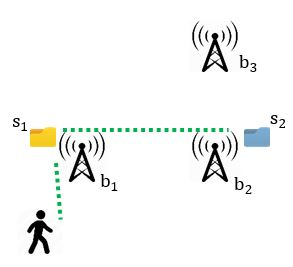
\includegraphics[width=0.7\linewidth]{figs/example_before.JPG}
		\caption{Service placement at $T_1$}
		\label{fig:alg_example_before}
	\end{subfigure}
	\hfill
	\begin{subfigure}[b]{.48\linewidth}
		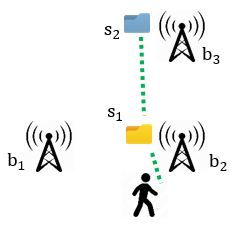
\includegraphics[width=0.7\linewidth]{figs/example_after.JPG}
		\caption{Service placement at $T_2$}
		\label{fig:alg_example_after}
	\end{subfigure}
	\vspace{\baselineskip}
	\caption{An illustrative example used for CMAB formulation}
	
	\label{fig:algo_example}
\end{figure}

\subsection{Bandit Formulation Example}
Assume there are $3$ base stations as shown in Fig.~\ref{fig:algo_example}. At time $T_1$, the user is in the vicinity of $b_1$. The first service $s_1$ is located in the edge server at $b_1$ and the second service $s_2$ is located in the edge server at $b_2$. Assume that after some time the user moves to the neighborhood of the base station $b_2$ at time $T_2$. As a result, he changes his service placement as shown in the  Fig.~\ref{fig:alg_example_after}. To get this placement, the user has selected the nodes at the base stations $b_2$ and $b_3$ ($n_1$ and $n_2$) as well as the links between himself and the base station $b_2$ and between base stations $b_2$ and $b_3$, which are referred to by $\ell_1$ and $\ell_2$. The unknown system parameter is expressed as follows:
\begin{align*}
	& \theta_{c}^{\intercal} = [\frac{1}{c_1}, \frac{1}{c_2}, \frac{1}{c_3}] \\
	& \theta_{b}^{\intercal} = [\frac{1}{b_{\ell_1}}, \frac{1}{b_{\ell_2}}, \frac{1}{b_{\ell_3}}, \frac{1}{b_{\ell_4}}] \\
	& \theta_{d}^{\intercal} = [d_{\ell_1}, d_{\ell_2}, d_{\ell_3}, d_{\ell_4}] \\
	& \theta_{\rho}^{\intercal} = [\rho_{e_1,e_2}^{s_1}, \rho_{e_1,e_3}^{s_1}, \rho_{e_2,e_3}^{s_1}, \rho_{e_1,e_2}^{s_2}, \rho_{e_1,e_3}^{s_2}, \rho_{e_2,e_3}^{s_2}] \\
	& \theta^{\intercal} = \theta_{c}^{\intercal} \oplus \theta_{b}^{\intercal} \oplus \theta_{d}^{\intercal} \oplus \theta_{\rho}^{\intercal}
\end{align*}
However, as the user does not know this parameter vector, starts with an estimate that is obtained by equations~\eqref{eqn:v_init}, \eqref{eqn:b_init}, and \eqref{eqn:theta_hat}-\eqref{eqn:delta_hat}.
Then, the user assumes $\hat{\theta}(t)$ is the correct parameter vector and use it to construct proper contextual feature vectors $\pmb{\chi}_{b_{2}}$ to compute the expected delays. Then, the user uses the computed expected delays to find the best chain placement. For example, the user, in order to evaluate the expected delay of the base station $b_2$ for placement of his first service $s_1$, uses the following contextual feature vector:
\begin{align*}
	& \pmb{\chi}_{b_{2}}^{c} = [0, \pi_{s_{2}}\lambda_{s_1}, 0] \\
	& \pmb{\chi}_{b_{2}}^{b} = [0, 0, 0, 0] \\
	& \pmb{\chi}_{b_{2}}^{d} = [0, 0, 0, 0] \\
	& \pmb{\chi}_{b_{2}}^{\rho} = [1, 0, 0, 0, 0, 0] \\
	& \pmb{\chi}_{b_{2}} = \pmb{\chi}_{b_{2}}^{c} \oplus \pmb{\chi}_{b_{2}}^{b} \oplus \pmb{\chi}_{b_{2}}^{d} \oplus \pmb{\chi}_{b_{2}}^{\rho}
\end{align*}
The user, then, uses the employed feature vectors and observed delay values to update the vectors $\pmb{V}_{t}$ and $\pmb{b}_{t}$ by using equation~\eqref{eqn:v_update} and \eqref{eqn:b_update}.

\subsection{Delay Estimation and Deployment Considerations}
\label{section:estimation}
Algorithm \ref{alg:cccpa} needs to know the contribution of each server and each link in the solution $O_{t}$ in the end-to-end delay (\ie\ $\{\delta_n(t)\}$). There are multiple hardware and software-based solutions to obtain these delays. Designing another mechanism for this problem is not the focus of this work. However, we briefly explain the viability of obtaining these estimates by employing current studies. A simple and lightweight approach is using time-stamped packets, where a special packet is sent along the same path that carries the service traffic. Each server adds a timestamp that specifies the packet's arrival time and another timestamp that specifies a departure time, which is set to be after the mean processing time of the service packets. A simple daemon that is deployed on servers can accomplish this task. In order to compute the mean service time for each service more precisely, it is possible to employ the approach that is presented in~\cite{koMON}. Further, it is possible to use available tools (\eg\ \cite{SDNTimeSyn}) to achieve the desired level of time synchronization that is enough for the accuracy of timestamped-based calculations. However, it is possible to employ the ideas from the network tomography, which is deeply studied, to avoid network synchronization complications and overheads. With approaches like~\cite{SLAM}, it is possible to obtain link-level delay estimates from end-to-end measurements. The processing delays can be obtained with the same approach as before, and the servers can directly send their measurements to the user.  

In chapter~\ref{chap:estimation}, we present our design of a simple timestamp-based estimation framework.

% \cat{Clock synchronization}
% \textit{Clock synchronization}\cite{clocksyn} is often an issue that is considered in distributed systems, however, in our deployment, all the servers are running as an virtual instance on one machine, thus we do not consider this issue in our paper.

% \cat{Network noise when collecting time stamps}
% When deploying the time-stamp estimation framework, we notice that the estimated delay is usually higher than the actual configured delay because of the noise delay in the network, that is, $\bar{d}_{n}(t) = d_{n}(t) + \epsilon_{n}(t)$, where $\epsilon_{n}(t) > 0$.


% \begin{figure}[t]
%     \centering
%     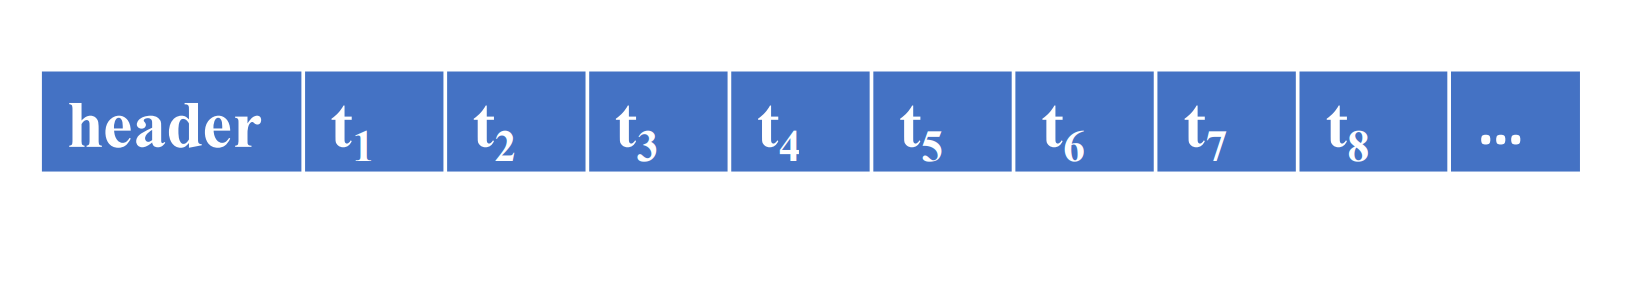
\includegraphics[width=0.9\linewidth]{figs/packetformat.PNG}
%     \caption{Estimation packet format}
%     \label{fig:estimation_packet_format}
% \end{figure}


% Notice that if the values of $x_{n}^{s}(t)$ and $y_{\ell}^{s}(t)$ are a feasible solution for the \myproblem problem, then $\sum_{n\in O_{t}} \delta_{n}(t)$ is the end-to-end delay. Next, we show how the system can collect the values of $\delta_{n}(t)$ (the delay incurred by using node $n$) in an efficient manner and send them back to the user. 

% In this section, we present our proposed Contextual combinatorial upper confidence bound algorithm (\cucb) for \myproblem. The basic idea of \cucb is to balancedly explore and exploit each arm in $\mc{A}$ by "adjusting" them before selecting. The algorithm performs as follow:

% During the learning slots, the algorithm will maintain: (1) variable $T_i$ as the total number of times arm $i$ is played so far; (2) variable $\hat{\mu}_i^t$ as the mean of all outcomes of arm $i$ observed so far, which will be used to adjust the estimation of each arm. 
% At each timeslot $t$, the algorithm first adjust each arm estimation and update the contextual information, which are then given to the oracle (denote as $\mc{O}$) as input.

% Then, the algorithm plays the super arm $S(t)$ returned by the oracle and uses the observed outcome to update $T_i$ and $\hat{\mu}_i^t$, while receiving an actual cost.
% The pseudo-code of the algorithm is summarized in algorithm \ref{alg:CMAB}.

% In step5, we apply an adjustment term to each arm estimation as follow:
% where $\hat{\mu}_i^t$ is the average estimate of arm $i$ so far at timeslot $t$,  $T_i$ is the number of times arm $i$ has been selected, by doing such adjustment we are performing what's called Upper Confidence Bound Selection\cite{UCB}, which uses uncertainty in the arm-value estimates for balancing exploration and exploitation, e.g. For those arms that have not been selected much times, its $T_i$ will be smaller and $\bar{\mu}_i^t$ will be smaller, this will increase the chance of arm $i$ being "explored". Moreover, $c$ decides the level of exploration, the bigger $c$ is, the more likely it is to explore a less selected arm, by doing this, we either gets the highest reward or we get to learn about an arm that we know least about.


%\subsubsection{Capacity measurement 1}
%Now we introduce two techniques for computing capacity and link capacity measurement respectively.
%For a reliable processing delay estimation on a computing node,  we apply $KOMon$ \cite{koMON} framework to measure the packet times of VNF through lightweight in-stack monitoring.

%For measuring link bandwidths along a path, we apply $pathchar$ \cite{jacobson1997pathchar}, $pathchar$ is a measurement tool developed by Van Jacobson at Lawrence Berkeley Laboratory (LBL), that can be used to find the bandwidth, delay, average queue and loss rate of every links in the network.

%$pathchar$ utilize the time-to-live (ttl) field of a IP packet, ttl  limits how many links it can traverse in the network before it expires, e.g. if a router receives an expired packet, it sends an ICMP error packet back to the sender, therefore the address of the $n$th router can be found by setting ttl to a value $n$. $pathchar$ works by sending probes with different ttl values and different sizes, it measures the time of each probes until the error packet returns, then it analyze the returned data based the following rtt formula from two nodes (say $n$ and $n-1$) using Van Jacobson's specifications:

%\begin{equation}
%\begin{aligned}
%   rtt &= q_1 + (latency + packet\_ size/bandwidth) + q_2 + forward \\   &   +q_3 + (latency + error\_size/bandwidth) + q_4,\\
%\end{aligned}
%\end{equation}

%where $q_i$ are random variables that represent the queuing delays between nth and n-1th node, $forward$ is the packet processing time when forwarding the packet. But $pathchar$ assumes three things: (1) the size of the error packet is negligible, (2) the forwarding time is negligible and (3) the queuing delays are negligible if enough measurements are made on a given path. Therefore we have:

%\begin{equation}
%   rtt = (latency + packet\_size/bandwidth) + latency.
%\end{equation}
%In our case, we apply the following probing steps on a SFC path to get the estimation of link latency and processing delay :
%\begin{enumerate}
%   \item At each timeslot, send multiple probe packets simultaneously to the $n$ nodes on the SFC path with various packet sizes, it then measures the round trip time (rtt) until a feedback packet is received, denoted by $rtt_n$
%  \item Each server i, upon receiving the probing packet, sends back a feedback packet with processing delay measured by KOMon(e.g. queue size), which will be used as processing capacity estimation. 
%   \item Analyze the feedback packet based on $pathchar$ and reconstruct link-by-link path characteristic
%\end{enumerate}
%A round trip time to node $n$ can for packet of size $s$ be expressed as
%\begin{equation}
%    rtt_n = \sum_{i=1}^n[s/b_i + d_i/c] + 2*\sum_{i=1}^n f_i
%\end{equation}
%A example for packet routing and probing in SFC placement is shown in figure 6.
% %\begin{figure}
%  %   \centering
%   %  \includegraphics[width=0.7\textwidth]{pathchar.PNG}
%     \caption{SFC packet routing and probing}
%     \label{fig:my_label}
% \end{figure}


% For analysis, we assume that the probing packet is small enough so that the processing delay and queuing delay can be negligible, therefore we have:
% \begin{equation}
%     rtt_n = 2*\sum_{i=1}^n f_i, n\in \mathcal{S}.
% \end{equation}

% \subsubsection{Capacity measurement 2}
% For processing delay measurement, using KoMON\cite{koMON}, for each computing node, upon receiving the first packet in a SFC request, it starts to calculate the processing delay and send it back to user after processing the last packet of SFC request. Processing delay piggy back packet will then be using the same timeslot as the SFC request. More specifically, the server doesn't have to know the exact timeslot, it just need to make sure that a task is finished and processing delay is calculated within a time interval, say $\tau$

% For processing delay, we apply SLAM\cite{SLAM} framework that is designed for SDN, SLAM is deployed on centralized controller and combines four components: rule generator, traffic generator, traffic listener, and latency estimator (as shown in Figure ). The latency computation process is composed of three steps: 
% \begin{enumerate}
%     \item  Preselect end-to-end path and install specific flow monitoring rules on all switches along the path. 
%     \item Controller sends constructed probe packets that match monitoring rules to switches and then the probe will traverse through the monitored path. Once the probe packet arrived at a switch, it will be regarded as a new flow and trigger Packet\_in message to controller. 
%     \item  Controller estimates path's latency based on the time-stamp in these messages. 
% \end{enumerate}


%currently 
% Now we introduce our $Capacity\ Update\ Protocol$ for measuring link capacity in one hop. it uses a simple timestamp insertion to the probing packet for the calculation of end-to-end delay from one computing node to another and the computing delay on a computing node. As depicted by Figure 6, each node inserts current time as a timestamp to the probing packet before sending it to the next node , while it also keeps track of time when processing the request. e.g., for a request with $\lambda^t$, Node A sends the request to Node B at $t_1$, Node B receives it at $t_2$ and finish the request at $t_3$, link capacity $LC$ and computing capacity $CC$ is then calculated by:
% \begin{equation}
%     LC = \lambda^t/(t_1-t_2),\  CC=\lambda^t/(t_3-t_2),
% \end{equation}
% In order to solve the issue that the system clocks of two edge nodes are usually not synchronized, we use $packet\ pair\ probing$\cite{1049160} that can give us a better estimation of link capacity. 
% Consider the scenario that Packet i arrives at link($A\rightarrow B$) at $\tau_i$ and leaves the link at $\tau^*_i$, the link delay is therefore 
% \begin{equation}
%     d_i = \tau^*_i - \tau_i = \lambda^i/LC, 
% \end{equation}
% We compare two adjacent packet we have:
% \begin{equation}
% \begin{aligned}
%     \text{inter-arrival time:}\ t_i&=\tau_i - \tau_{i-1}, \\
%     \text{inter-departure time:}\ t^*_i&=\tau^*_i - \tau^*_{i-1},\\
%     \text{delay variation:}\ \delta_i &= d_i - d_{i-1}=t^*_i-t_i\\
%     &=\lambda_i/LC - \lambda_{i-1}/LC\\
%     &=(\lambda_i-\lambda_{i-1})/LC.\\
%   \end{aligned}
% \end{equation}
% Therefore we have:
%     \begin{equation}
%         LC = (\lambda_i-\lambda_{i-1})/(t^*_i-t_i).
%     \end{equation}
% With packet pair probing we are able to calculate link capacity by using the interval between a packet pair that is not affected by the clock offset.

% For a more reliable processing delay estimation on a computing node,  we apply $KOMon$ \cite{8854514} framework to measure the packet times of VNF through lightweight in-stack monitoring. 


% \begin{figure}
%     \centering
%     \includegraphics[width=0.7\textwidth]{timestamp.PNG}
%     \caption{Delay Update Protocol (DUP)}
%     \label{fig:my_label}
% \end{figure}


% \subsection{Message Complexity Analysis}
% In our proposed framework we use the commonly deployed Transmission Control Protocol (TCP) as a measurement service. We now analyze the complexity of estimation packet.
% %In order to support the need for $KOMon$, we assume that all the computing nodes has KOMon module loaded into its kernel beforehand.  

% \subsubsection{Packet size}
% As we described before in packet format, each estimation packet requires $(l+1)*18$ bytes for storing information time stamps for a SFC of length $l$. Therefore a TCP based packet size will be:
% \begin{equation}
% \label{eqn: packet size cal}
%     20 + (l+1)*18 = 38+18l
% \end{equation}
% bytes in total with 20 bytes for the TCP header. As it may be concerned, here we do not consider the issue of clock synchronization\cite{clocksyn} due to the fact that all of our emulation experiments will be executed on virtual computing machines that are in the same time system. 

% \subsubsection{Number of packets sent in each timeslot}
% As it may be apparent, assume that $n$ packets are sent to measure each link bandwidth on a SFC, the number of packets sent in total can be calculated by:
% \begin{equation}
%     N = 1 + n*s,
% % \end{equation}
% where $s$ is the number of links on a SFC path.




% Explain how many packets (how many bytes) will be sent to collect estimated information. 

% TCP/IP header overhead discussion. 
% You are designing the body of the messages. 
% But, you use TCP/IP (or even UDP) to send them. 

% How many request packets will be sent in a single timeslot?
% How many response packets will be sent in a single timeslot?

% Processing delay measurement is easy.
% ** IMPORTANT **
% "How to measure link delays?"
% Link delay measurement
% Link delay monitoring
% Per-link delay estimation


%To mitigate the measurement uncertainty and obtain a robust placement that is able to handle system dynamics we design our algorithm based on the contextual combinatorial bandit problem. 


%  Where $C()$ and $P()$ is the combination and permutation function respectively. 

% At the beginning of the arm selection, only the user side information is known, such as user's location and user's request, which are used as the context information. The information about the nodes are unknown, but as learning slots proceeding and arms being chosen, the system may gain a better knowledge of the arms and make better decisions based on it. 

% The selection is made in a way that is shown in Figure \ref{fig: selectionmakingdiagram}. In each timeslot the user selects the same number of computing nodes that equals to the services as an arm to deploy the SFC, and then they send their traffic towards SFC and waiting for the task to be processed. Due to the mobility, the users may or may not change the nodes to place each service on.
% \begin{figure}
%     \centering
%     \includegraphics[width=0.9\linewidth]{system.PNG}
%     \caption{Selection making during two timeslots}
%     \label{fig: selectionmakingdiagram}
% \end{figure}
% % ========== END examples

% Based on the descriptions above, We now transform the SFC problem into a general Contextual CMAB. To better formulate the SFC placement into a multi-arm bandit problem, we first characterize each computation node $i$ using a feature vector $\mu$ and then the super arm set $\eta$ will be formulated based on the node feature vector and the service number in SFC, which has size $n$ calculated in (7). 

% \begin{equation}
% \begin{array}
%     % &\mu_i^t = [1/c^t_i, f^t_{i, 1}, ..., f^t_{i, n}],\\
%     &\eta = \{\eta_1, \eta_2, ..., \eta_N\},\\
%     &\eta^t = [\mu_1^t, ..., \mu_s^t].\\
%   \end{array}
% \end{equation}
% where $\eta^t$ is the arm set that is selected at timeslot $t$ and $\mu_s^t$ denotes the node that runs service $s$ at timeslot $t$.

%  \begin{algorithm}
% \caption{Contextual MAB}
% \begin{algorithmic}[1]
%  \renewcommand{\algorithmicrequire}{\textbf{Initialization:}}
%  \renewcommand{\algorithmicensure}{\textbf{Online Learning}}
%  \REQUIRE \ 
%   \STATE Initialize the cumulative context of each super arm $\eta_i$ in set $\eta = \{\eta_1, \eta_2, ..., \eta_n\}$, $B_i = \textbf{I}$ ($s*(2M+3)$ dimensional identity matrix), the estimated vector of each super arm: $\hat{\eta_i} = \textbf{0}$ ($s*(2M+3)$ dimensional zero vector), cumulative SFC cost of super arm $\eta_i$: $f_{\eta_i} = \textbf{0}$ 
%  \ENSURE  \
%   \FOR{each timeslot $t = 1,2,...,T$}
%   \STATE  \textbf{Sample} the aggregated cost $\theta_{\eta_i}(t)$ for each super arm $\eta_i$ from the posterior distribution $\mathcal{N}(b(t)^{\top}\hat{\eta_i}, v^2b(t)^{\top}B_{\eta_i}^{-1}b(t))$
%   \STATE \textbf{Select} the super arm $s(t) = argmin\theta_a(t)$ and receive an actual cost $r_t$
%   \STATE \textbf{Update} $B_{s(t)} = B_{s(t)} + b(t)b(t)^{\top}, f_{s(t)} = f_{s(t)} + b(t)r_t, \hat{\eta_s} = B^{-1}_{s(t)}f_{s(t)}$
%   \ENDFOR
%  %\RETURN $P$ 
% \end{algorithmic} 
% \end{algorithm}

%  Where $\lambda^t$ indicates the current SFC demand, $g^t$ indicates the current user location and $f^t$ records the last SFC placement. 

%  $v$ is a control parameter in algorithm 1.


% In this subsection we present how to transform the SFC placement problem in to a general contextual CMAB problem.


% For a network with $m$ nodes, We define the links as an arm set $\mathcal{L} = \{\ell_1^t, \ell_2^t, ...., \ell^t_m \}$, where $\elll_i^t$ represent the link set from node $i$, thus we have:
% \begin{equation}
%      \mathcal{L} = \{\ell_1^t, \ell_2^t, ...., \ell^t_m \}, \ \
%      l^t_i = \{f^t_{i,1}, f^t_{i,2}, f^t_{i,3}, ..., f^t_{i,m}\},
% \end{equation}


% where $f^t_{i,j}$ denotes the link attribute from node $i$ to node $j$ at timeslot $t$ (e.g. transmission delay). We then define the link arm set as a binary vector $X^t = [x^t_{1,2},...,x^t_{1,m},x^t_{2,1},...,x^t_{2,m}, ..., x^t_{m,1}, ..., x^t_{m,m}]$ for selection, where $x^t_i = 1$ means link arm $i$ is chosen.
% Computing nodes are defined as a arm set $\mathcal{N} = \{ c_1^t, c_2^t, ..., c_m^t\}$, where $c_m^t$ represents the computing capacity on node $n$. Again we define the node arm set as a binary vector $Y^t = [y_1^t, ..., y^t_m]$ for selection, where $y^t_i = 1$ means node arm $i$ is chosen. 


% Estimation of the single arms and collecting those estimations at the user-side for further placement decisions is explained in detail in section~\ref{section:estimation}. 


% \subsection{Arms formulation in \myproblem}
% The arms in our problem are a collection of links and nodes, that is, $\mc{A} = \mc{N}\cup\mc{L}$, where $\mc{N}$ denotes the set of all node arms, $\mc{L}$ denotes the set of all link arms and we use $\mc{A}$ to denote the set of all arms.
% We then further transform both link arms and node arms into aforementioned binary vector for section, denoted by $X^t$ and $Y^t$, therefore we can express the arm formulation for \myproblem as follow:
% \begin{equation}
%     \begin{aligned}
%       X^t &= \{x^s_n(t)\}.\qquad \forall n\in\mc{N}, s\in \mc{S}, t\in\mc{T}\\
%       Y^t &= \{y^s_\ell(t)\}.\qquad \forall \ell\in\mc{L}, s \in \mc{S}, t\in\mc{T}\\
%     \end{aligned}
% \end{equation}
% At each timeslot, the user need to decide a set of arm to deploy the current SFC, we denote it by $\mc{S}(t)$, the super arm consist of the node and link arms selected to place this SFC. Formally, the super arm can be expressed as:
% \begin{equation}
%     \begin{aligned}
%       & S_t  = \{x^s_n(t), y^s_\ell(t)\}_{s\in\mc{S}(t)}

%     \end{aligned}
% \end{equation}
% where
% \begin{equation}
%     \begin{aligned}
%       &  \sum_{n\in\mc{N}} x_{n}^{s}(t)  = 1. 
%     \qquad 
%     \forall s\in\mc{S}, t\in\mc{T}\\
%     &\sum_{s\in\mc{S}} x_{n}^{s}(t) \le 1. 
%     \qquad 
%     \forall n\in\mc{N}, t\in\mc{T}\\
%     \end{aligned}
% \end{equation}


% Similar to many existing works \cite{MABserviceplacement, Mobility-Aware},
% Specifically, computing delay is calculated from arm set $X$ while migration and transmission delay is calculated from arm set $Y$. Therefore we define the reward function at each timeslot to be:
% where $d^t_{cp}$, $d^t_{cm}$ and $s^t$ are the computing delay communication delay and switching cost respectively. Specially, our switching cost will be calculated from a general model that is based on link capacity and the size of the VNF that needs to be migrated, we have:
% \begin{equation}
%     s_{i,j}^t = \alpha \cdot  \lambda_{S_i}^t /f_{i,j}^t,
% \end{equation}
% where $\alpha$ is an adjustment coefficient, $\lambda_{S_i}$ represents the size of the VNF that provides service $S_i$. 
% \subsection{Reward function of a super arm}
% We define our reward function to be the objective of \myproblem, that is, the end-to-end delay perceived by user, which is mainly consist of three parts as formulated in section \ref{section: formulation}: computing delay, transmission and propagation delay, migration delay. 
% As defined before, the reward function of a super arm $S$ at timeslot $t$ can be expressed as:
% \begin{equation}
%     \begin{aligned}
%          r(S_t) &= \text{Min. } \sum_{i=1}^{4} \gamma_{i}\Gamma_{i}(t)
%     \end{aligned}
% \end{equation}


%
% To consider user's specific context such as mobility and requests, we define the current-time-slot information such as user's connected base station $\beta(t)$, SFC request $\Lambda(t)$ and previously selected super arm $S_{t-1}$ as the contextual information, denoted by $\mc{C}(t)$, which is expressed by:
% \begin{gather}
%     \mc{C}(t) = [\beta(t), \Lambda(t), S_{t-1}], \\
%     \Lambda(t) = [\lambda_{s_1}(t), ..., \lambda_{s_k}(t)], \\
%     S_{t-1} = \{x^s_n(t-1), y^s_\ell(t-1)\}_{s\in\mc{S}(t-1)}.
% \end{gather}


%
% In order to treat each arm individually and be able to use their information that can be observed when playing a super arm for further selection, we formulation each link and node as individual arms. More specifically, we assume that we are able to get an estimation of each link and node by time-stamp techniques that are introduced in section~\ref{section:estimation}.
% %
% We then define the super arm selection policy that constraints the combination of links and arms to be physically feasible in a network, and the context information used for selection. 

% \subsection{Arms formulation in \myproblem}
% We then further transform both link arms and node arms into aforementioned binary vector for section, denoted by $X^t$ and $Y^t$, therefore we can express the arm formulation for \myproblem as follow:
% \begin{equation}
%     \begin{aligned}
%       X^t &= \{x^s_n(t)\}.\qquad \forall n\in\mc{N}, s\in \mc{S}, t\in\mc{T}\\
%       Y^t &= \{y^s_\ell(t)\}.\qquad \forall \ell\in\mc{L}, s \in \mc{S}, t\in\mc{T}\\
%     \end{aligned}
% \end{equation}
% At each timeslot, the user need to decide a set of arm to deploy the current SFC, we denote it by $\mc{S}(t)$, the super arm consist of the node and link arms selected to place this SFC. Formally, the super arm can be expressed as:
% \begin{equation}
%     \begin{aligned}
%       & S_t  = \{x^s_n(t), y^s_\ell(t)\}_{s\in\mc{S}(t)}

%     \end{aligned}
% \end{equation}
% where
% \begin{equation}
%     \begin{aligned}
%       &  \sum_{n\in\mc{N}} x_{n}^{s}(t)  = 1. 
%     \qquad 
%     \forall s\in\mc{S}, t\in\mc{T}\\
%     &\sum_{s\in\mc{S}} x_{n}^{s}(t) \le 1. 
%     \qquad 
%     \forall n\in\mc{N}, t\in\mc{T}\\
%     \end{aligned}
% \end{equation}


% \subsection{Policy for choosing a Super arm}
%  To satisfy the requirements of a SFC when choosing a super arm, we use the routing constraint and link constraint introduced in section \ref{section: formulation} as the policy of choosing super arms:

% \begin{equation}
% \label{eqn: superarmpolicy}
% \begin{aligned}
%   & \sum_{\ell\in\delta^{+}(r)} y_{\ell}^{s_{i}}(t)
%     - \sum_{\ell\in\delta^{-}(r)} y_{\ell}^{s_{i}}(t)
%     = x_{n_r}^{s_{i}}(t) - x_{n_r}^{s_{i+1}}(t).\\
%     &\qquad\qquad\qquad\qquad\qquad\qquad\qquad\forall r \in\mc{R}^{'},t\in\mc{T}\\
%     &\sum_{s_{i}\in\mc{S}} \lambda_{s_{i+1}}(t)y_{\ell}^{s_{i}}(t) \le b_{\ell}(t).
%       \qquad\forall \ell\in\mc{L}, t\in\mc{T}\\
% \end{aligned}
% \end{equation}
%  We assume that the SFC path always starts from user's current connected station and goes back to it, as shown in Figure 2.
% % \begin{equation}
% % \label{eqn: superarmpolicy}
% %     \begin{aligned}
% %     & \sum^{m}_{i=1}\sum^{m}_{j=1}x_{i,j}^t = \sum^m_{i=1}y_i^t, x_i^t \in X^t, y_i^t \in Y^t, \\
% %     & S^t = [c^t_g, f^t_{i,j}, c^t_j, f^t_{j,p}, c^t_p, ..., f^t_g], \\
% %     &\sum^m_{j=1}x_{i,j}^t=1, \sum^m_{j=1}x_{j,i}^t=1,  c_i^t \in \mathcal{N}.\\
% %     \end{aligned}
% % \end{equation}
% % where the first equation constraints the number of selected nodes should equal the number of selected links due to the SFC-to-user loop, the second equation requires that the selected nodes and links are able to form a path that returns to user, the third equation constraints that for any node selected for super arm, only one incoming and ongoing link arm will be selected. 
% This policy will be applied in the Oracle of the placement algorithm introduced in the next section.


% \begin{algorithm}
% \setAlgoLined
% \caption{\cucb}
% \label{alg:CMAB}
% \begin{algorithmic}[1]
%  \renewcommand{\algorithmicrequire}{\textbf{Initialization:}}
%  \renewcommand{\algorithmicensure}{\textbf{Online Learning}}
%  \REQUIRE \ 
%   \STATE For $i \in \mc{A}$ , maintain: (1)variable $T_i$ as the total number of times arm $i$ is played so far; (2) variable $\hat{\mu}_i^t$ as the mean of all outcomes of arm $i$ observed so far.
%   \STATE For each arm $i \in \mc{A}$, get a initial estimation $\hat{\mu}_i^0$ and set $T_i$ to 1.   
%   \STATE Initialize contextual $\mc{C}(1) = [\beta(1), \Lambda(1), S_0]$
%  \ENSURE  \
%   \FOR{$t \leftarrow 1,2,...,T$}
%     \FOR {$i \in \mc{A}$}
%     \STATE$\bar{\mu}_i^t \leftarrow \hat{\mu}_i^t - \sqrt{ \frac{3\ln t}{2T_i}}$.
%     \ENDFOR
%   \STATE $\mc{C}(t)\leftarrow [\beta(t), \Lambda(t), S_{t-1}]$
%   \STATE $S_t \leftarrow \mc{O}(\mc{C}(t), \{\bar{\mu}_1^t\}_{i\in\mc{A}}) $.
%   \STATE Select super arm $S_t$ and observe $\{\mu_i^t\}_{i\in{S_t}}$
%   \STATE Receive an actual cost $r(S_t)$
%   \STATE Update all $T_i$'s and $\hat{\mu}_i^t$'s, 

%   \ENDFOR
%  %\RETURN $P$ 
% \end{algorithmic} 
% \end{algorithm}


%  \begin{algorithm}
% \caption{DP-based oracle}
% \label{alg: oracleDP}
% \begin{algorithmic}[1]
%  \renewcommand{\algorithmicrequire}{\textbf{Input:}}
%  \renewcommand{\algorithmicreturn}{\textbf{Output:}}
%  \renewcommand{\algorithmicensure}{\textbf{Oracle:}}
%  \REQUIRE \ 
%   \STATE Adjusted arm estimation $\{\bar{\mu}_i^t\}_{i\in\mc{A}}$.
%   \STATE Context $\mc{C}(t) \leftarrow [\beta(t), \Lambda(t), S_{t-1}]$,
%  \ENSURE  \
%  \STATE Initialize $H(i,j) \leftarrow \mathbf{0};\quad \forall i\in \mc{S}[t], \forall
%  j\in \mc{N} $
%  \STATE Initialize $\text{Cost}(i,j)\leftarrow 0;\quad \forall i\in \mc{S}[t], \forall
%  j\in \mc{N}$
%   \FOR{$i = | \Lambda(t)|\to 0$}

%   \FOR{$j \in \mc{N} $}

%         \STATE  Compute and update $\text{Cost}(i,j), k$ according to eq.22-24
%         \STATE $H(i,j) \leftarrow H(i-1, k).append(k)$ 

%   \ENDFOR

%   \ENDFOR
%   \STATE Extract the node with the minimum cost to place vnf 1: $n \leftarrow \text{argmin}\{\text{Cost}(1, j)\}_{j \in \mathcal{N}}$

%   \STATE Get the corresponding host list as the super arm $S_t \leftarrow H(1, n)$
%  %\RETURN $P$ 
%  \RETURN Super arm $S_t$


% \end{algorithmic} 
% \end{algorithm}
%  \subsection{Time complexity}
%  The dynamic approach described in the oracle above is summarized in algorithm \ref{alg: oracleDP}, which results in a time complexity of $O(sn^2)$  with $n$ nodes and $s$ services, that is a bearable algorithmic time.


%All delays above can be calculated from the input arm estimation, .
%  In our CMAB algorithm, the oracle we used is a geo-ranged $argmin$ function (with $\alpha=\beta=1$) that is shown in Algorithm 3.

%  \begin{algorithm}
% \caption{SFC placement oracle}
% \begin{algorithmic}[1]
%  \renewcommand{\algorithmicrequire}{\textbf{Input:}}
%  \renewcommand{\algorithmicensure}{\textbf{Oracle}}
%  \REQUIRE \ 
%   \STATE Arm estimation vector $\hat{\mu} = [\bar{\mu}_1^t, \bar{\mu}_2^t, ..., \bar{\mu_m}^t]$.
%   \STATE Context vector $b(t) = [\lambda^t, g^t, F^{t-1}]$,
%   \STATE Current round time $t$, 
%   \STATE Selection range $r$.
%  \ENSURE  \
%   \FOR{each computing node $n$ within $r$ distance from $g^t$}
%   \STATE add it to the candidate list $C$
%   \ENDFOR
%   \STATE \textbf{LIST} all the subsets with the size equals to $\lambda^t$ from $C$

%   \STATE \textbf{COMPUTE} the cost $Cost_s(t)$ each subset $s$ in $C$, and set the subset with the least cost as the super arm.
%  %\RETURN $P$ 
% \end{algorithmic} 
% \end{algorithm}


% \begin{figure}
%     \centering
%     \includegraphics[width=0.9\linewidth]{oracle.PNG}
%     \caption{Oracle in SFC placement}
%     \label{fig:oracle}
% \end{figure}

% In SFC placement, the oracle limits that the selected nodes and links are able to be connected and formed into a complete SFC path. The selection of the exact optimal SFC path can be computationally hard and the learning algorithm may have a small failure probability. Thus, we resolve to the following $(\alpha,\beta)$-approximation oracle\cite{chen2013combinatorial}: For some $\alpha, \beta \leq 1$ that takes an expectation vector \texbf{$\mu$} as input, and outputs a super arm S such that :
%  \begin{equation}
%      Pr[r_{\mu}(S) \geq \alpha \cdot r_{\mu}(S_{opt})]\geq\beta
%  \end{equation}
%  Here $r_{\mu}()$ is the reward function, $S_{opt}$ is the exact optimal super arm and $\beta$ is the success probability of the oracle.


% $Oracle$ in the algorithm works as a super arm selection policy, it takes the estimates of individual arms as input and output a super arm for placement, as already mentioned before, it will follow the constraints in (11) when generating an super arm. More specifically, it explore all the nodes within a certain distance from user's current location and calculate the optimal combination of individual arms in terms of service cost based on the estimation.
% Contextual information $b(t)$ is also required in our algorithm and is formulated as (11). 


%
% \subsection{Related work}
% Probing techniques have been well study in the literature, we introduce two approaches: \cite{article, alizadeh2014conga} propose two different method of probe in order to get the link information, and use them in routing and load balancing respectively.
%
% In \cite{alizadeh2014conga}, the author present Conga, which focuses on the measurement of a link load, the idea of this method to measure a link between two nodes is to send packets and create a feedback loop between the sender and receiver to populate the metrics through the link. To store and estimate the metrics, they use DRE (discounted rate estimator), which maintains a register $X$, that is incremented for each packet sent over the link by the packet size in bytes, and is decremented periodically with a multiplicative factor $\alpha$ between 0 and 1: $X = X\times(1-\alpha)$. 
% the metric that needs to be measured in their case is congestion between two nodes.
%
% HyMAB \cite{article}
% on the other hand, focus on the strategy of finding a optimal multipath for a single flow in routing problem in order to get an optimal throughput. They proposed algorithm HyMAB, which treats each multi-path as arms, each time they choose one multipath to probe and get a reward. the arm is chosen based on a multi-arm bandit strategy that are introduced in \cite{auer2002finite}.
%
% After a arm is chosen which means the multipath is given, they compute an optimal rate on this path by solving a max rate linear problem.
% Now we present our time-stamp based estimation framework in SFC placement to measure the processing delays on each computing node and the transmission delay on each link. %Estimation of these two metrics will be stored in a SFC capacity vector (denoted by $E$) that returns to user along with the SFC response.


% Depending on the length of SFC, say $l$, each estimation packet would occupy $(l+1)*18$ bytes of payload to store all the time stamps because each time stamps takes 18 bytes to store in our implementation.
% \begin{itemize}
%     % \item \textbf{$nid_i (2 bytes)$}: this field is used by the nodes along the path to store the node id of the $i$th node in the SFC.
%     \item \texbf{$\Lambda_i(4bytes)$} : this field is used to store the size of SFC packets
%     \item \textbf{$t_i(4bytes)$}: link capacity, this field is used to store the time stamp.
%     % \item \textbf{DT}: Delay Table, This is a M-M table that stores the transmission delays in the networks at timeslot t, specifically for a node i, $T^t_i = [g^t_{i,1}, g^t_{i, 2}, ..., g^t_{i, M}]$, this table will be maintained by destination node based on index: SN and DN, one transmission delay metric will be inserted in this table after destination node receive the probe packet and calculate a delay.    
% \end{itemize}


% We apply an adjustment term to values obtained from above to encouraging exploring for the future rounds. For each link delay and computing delay we estimate from a SFC response, we can record the times of the same element that has been updated, for element $i$, we denote the total number of times it's been updated as $T_$ and apply the following adjustment:
% \begin{equation}
% \label{eqn:adjustment}
%     \bar{\mu_i} = \hat{\mu_i} - e * \sqrt{ \frac{3\ln t}{2T_i}},
% \end{equation}
% where $t$ is the current round number, $e$ is a configurable constant.


% \subsection{Oracle}
% \label{section: oracle}


%\section{Estimation of single arms}


% \subsubsection{Delay feedback}
% We use a feedback loop between the source node and the destination node for us to gain estimations for Computing capacity vector and transmission delay table. The probing process is described as follow:
% \begin{enumerate}
%     \item The source node first sends the probe packet to MEC network with the $nid_1$ field set to its node id and $c_i$ set to its computing capacity. 
%     \item As the packet routing through the MEC, each nodes it passes will calculate the link capacity from the last node before it process the packets and add it to f field, it also calculates it own computing capacity and insert it into $C^t$ vector in CC field.
%     \item When the packet is received at the destination node, it will add its transmission delay from last node to the TD field which will be the delay estimation from source node to destination node. Then it will add its computing capacity to the CC field and prepare for piggyback.
%     \item when a packet is sent in the reverse direction, the aggregated delay metric will be inserted to the delay table based on the source node id in SN field and destination node id.
%     \item Finally, the source node received and parse the piggyback packet and get a partial estimation of capacity vector and delay table.
% \end{enumerate}
%\subsection{SFC feedback}
%\subsubsection{SFC-to-user feedback loop}
%In our user-based SFC problem, we use a SFC-to-user feedback loop to obtain the network information. Explicitly we assume that probing process is within the SFC process, that is, when the SFC request is roaming through the VNFs (virtual network functions), the estimation packet will also be passed on the nodes that has the VNFs placed on along with the SFC packets. In the end of a timeslot, the user will not only receive a SFC response but also an updated estimation vector, this process is illustrated in figure 5.
%\begin{figure}
%    \centering
%   \includegraphics[width=0.7\textwidth]{probingservicechain.PNG}
%  \caption{Probing in SFC placement}
% \label{fig:my_label}
%\end{figure}


% Especially for processing delay, the error might be amplified by the size of the processing packet.


% The basic steps of DP can be summarized as follow:
% \begin{itemize}
%     \item characterizing the structure of an optimal solution
%     \item Defining the cost of an optimal solution recursively
%     \item Computing the cost of an optimal solution in a bottom-up fashion
% \end{itemize}


% \begin{equation}
%      \bar{\mu}_i^t = \hat{\mu}_i^t - c* \sqrt{ \frac{3\ln t}{2T_i}}, 
% \end{equation}


% However, the formulation in general CMAB yields an exponential number of arms as shown in equation \ref{eqn:number of super arms}, which may have computational limitations and this approach of forming super arms will also neglect the information of single arms that can be observed from the outcomes received after choosing a super arm.


% \theta_{n} = [\frac{1}{c_{n}}(t), \rho_{a,b}^{s}(t)]^{\intercal} \\
% \chi_{n}^{s_i}(t) = [\pi_{s}\lambda_{s}(t), x_{b}^{s}(t-1)]^{\intercal} \\
% \theta = [\theta_{n}]^{\intercal} \\
% \chi_{n}(t) = [\chi_{n}^{s_1}(t),\dots,\chi_{n}^{s_S}(t)] \\


% Note that the propagation delay of a link is a function of distance and does not depend on the location of the user or the placement of the services. Thus, for each link $\ell$ the delay $\delta_{\ell}(t)$ is simply defined as,
% \begin{gather}
%     \delta_{\ell}(t) = d_{\ell}(t) + \epsilon_{n}(t).
% \end{gather}


% In this section we present our proposed CMAB formulation for \myproblem and then we introduce a contextual combinatorial upper confidence bound ($\text{C}^2\text{UCB}$) algorithm with a Dynamic Program (DP) based oracle that solves the CMAB problem.


% \begin{algorithm}[t]
%     \DontPrintSemicolon
%     \caption{RL-based chain allocation}
%     \label{alg:CMAB}
%     \SetKwInput{kwInit}{Init}
%     \KwIn {$\lambda$, $\{\pmb{\chi}_{n}(0)\}$}
%     \kwInit{}
%     \For{$t \in \mc{T}$}{
%         \For{$n \in \mc{N}$}{

%         }
%         $O_{t} \gets$ get\_alloc($\{\hat{\delta}_{n}(t)\}$, $\{\pmb{\chi}_{n}(0)\}$)
%         \hfill //See Alg. \ref{alg:get_alloc} \\

%     }
% \end{algorithm}


% In the following, we explain the definition of feature vectors and the approach of selecting appropriate set of servers and links for the placement of the service chain in each timeslot.


% To collect these information, we design a lightweight timestamp-based delay estimation and distribution framework to lower the overhead and facilitate deployability. 
% %
% To estimate delays in the network, {\color{red} This sentence is a bit vague, we should discuss it more: we time-stamp one packet and tag it along with the packets that we send for each SFC request while keeping track of the time.} The estimation framework has two parts:
% \begin{itemize}[leftmargin=*]
%     \item \textbf{An initial estimation of the whole network:} {\color{red} I think we can make this part more sophisticated... for example define a radius of servers that we recieve an estimation for them.} The user first sends a request to each computing node, upon receiving the request, the server will send packets to the other servers and time stamp them. After receiving all the returned packets, the server parse the time stamps in them, calculate the delays and send those information back to the user. The user collect all the delay estimations from the servers and save it as a initial estimation that is required in the CMAB algorithm.
%     \item \textbf{Estimation of delays on the chosen SFC path:} We also time-stamp the packets we send in each SFC request, after the packet is returned from the SFC, the user parses the time stamps and calculates the delays on the SFC. Those estimations will then be used to update the initial estimation in accordance with algorithm \ref{alg:CMAB}.
% \end{itemize}


% \cat{Example 2}
% Consider a SFC with three different services as an example. The formatting of the packet that's used for estimation is shown in figure \ref{fig:estimation_packet_format}, each server on the path append the time stamps to the packet during the service. 
% We consider a scenario that the VNFs are placed on node A, B, C at the moment and that user is connected to node D, as shown in figure \ref{fig:timestampsMEC}. The SFC request from a mobile user will be time stamped and recorded, as the request being handled on the chain, each processing node will time stamp the packet when it receives a packet and after the processing is done. The time-stamping process is described as follow:
% \begin{enumerate}[leftmargin=*]
%     \item  User generates SFC request packets with size $\lambda_i$ bytes for each service $i$, while inserting the current time to $t_1$ to the last packet.
%     \item Node A receives the request first in the SFC, upon receiving the last packet, it update the packet by inserting its current time $t_2$ and start processing the packets. When the processing is done, node A insert the current time $t_3$ to the same packet , then it sets the destination to node B as the next service handler and forward all the packets.
%     \item Node B process the second requested task and insert time stamp $t_4$, $t_5$ before and after the task respectively. Then it sets the destination to C and forward the packets.
%     \item Node C processes the last request, it repeat the time stamping ($t_6$, $t_7$) and send a SFC response along with a packet that stores all the time stamps in order.
%     \item Finally, the user receives the response for their services and a list of traversed time stamps while recording the current time $t_8$ upon receiving. 
% \end{enumerate}
% Based on the time stamps and SFC packet sizes, user are able to calculate the corresponding estimated link delay and processing delay as follow:
% \begin{equation}
%     \label{eqn:timestampcalculation}
%     \begin{aligned}
%     d_{D \rightarrow A} &= t_2 - t_1\\
%     d_{A \rightarrow B} &= t_4 - t_3\\
%     d_{B \rightarrow C} &= t_6 - t_5\\
%     d_{C \rightarrow D} &= t_8 - t_7\\
%     d_A           &= (t_3 - t_2)/\lambda_1\\
%     d_B           &= (t_5 - t_4)/\lambda_2\\
%     d_C           &= (t_7 - t_6)/\lambda_3\\
%     \end{aligned}
% \end{equation}

% \begin{figure}[t]
%     \centering
%     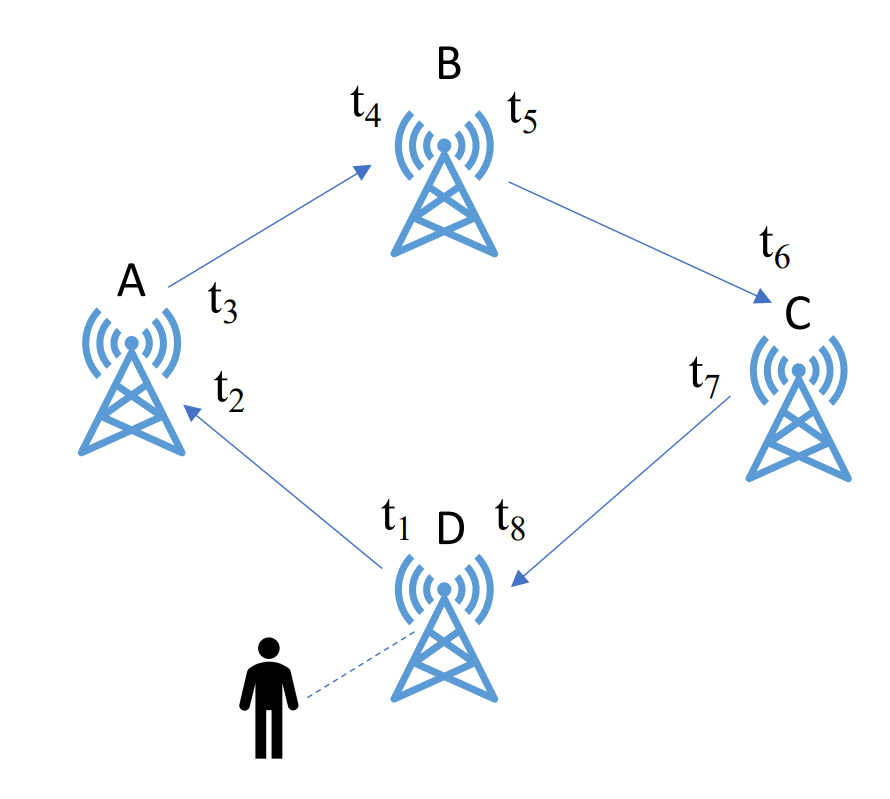
\includegraphics[width=0.9\linewidth]{figs/SFCtimestamp.PNG}
%     \caption{Time stamps of SFC placement in MEC}
%     \label{fig:timestampsMEC}
% \end{figure}


% We use the contextual combinatorial bandit framework to characterize the placement options that the user can choose from. This framework allows the user to employ the reinforcement learning and account for the relation between the perceived quality of service in terms of delay and the service type, traffic rate, and the mobility. Also,